\documentclass[a4paper,11pt]{article}
\usepackage{ucs}
\usepackage[utf8x]{inputenc}
\usepackage[english,greek]{babel}
\newcommand{\en}{\selectlanguage{english}}
\newcommand{\gr}{\selectlanguage{greek}}

\usepackage{verbatim}
\usepackage{amsmath}
\newcommand{\matr}[1]{\mathbf{#1}}
\usepackage{mathtools}
\DeclarePairedDelimiter\abs{\lvert}{\rvert}
\DeclarePairedDelimiter\norm{\lVert}{\rVert}

\usepackage{hyperref}
\usepackage{multirow}
\usepackage{enumitem}
\usepackage{graphicx}


\gr
\title{Εργασία 2}
\author{Όνοματεπώνυμο: Γεώργιος Δάγκαλης\\  ΑΕΜ: 3164}       
\date{\today}




\begin{document}
	\maketitle
	
	
	\section{Γενικά}\label{ux3b3ux3b5ux3bdux3b9ux3baux3ac}
	
	\gr Ο κώδικας της εργασίας υλοποιήθηκε στην γλώσσα προγραμματισμού \en python. \gr Μέσα στο αρχείο \en main.py \gr υπάρχει ο κώδικας για την Άσκηση \en 5(1 \gr και \en 3 \gr υποερωτήματα) και για την άσκηση \en 7. \gr Το παρόν παραδοτέο χωρίζεται σε δύο μέρη. Στο πρώτο μέρος επεξηγείται η λειτουργία του κώδικα και στο δεύτερο μέρος περιγράφονται οι λύσεις των ασκήσεων και τα αποτελέσματα τους.
	
	
	\section{Υλοποίηση}\label{ux3c5ux3bbux3bfux3c0ux3bfux3afux3b7ux3c3ux3b7}
	
	\subsection{\en Main}\label{main}
	
	\gr Από εδώ ξεκινάει η εκτέλεση του κώδικα. Ο κώδικας συνολικά έχει φτιαχτεί έτσι ώστε να μπορούμε με το κάλεσμα μιας συνάρτησης να μπορούμε να πάρουμε το αποτέλεσμα ενός ερωτήματος μέσα στην εργασία. Μέσα στην \en main \gr υπάρχουν οι συναρτήσεις που λύνουν κάθε ερώτημα μέσα σε \en comment \gr έτσι ώστε να μην μπερδέυονται τα αποτελέσματα μεταξύ του και να μην μπλοκάρει το ένα \en plot \gr το άλλο.  \textbf{Προσοχή:} Κατά την διάρκεια ένός \en plot \gr η εκτέλεση του κώδικα σταματάει σε εκείνο το σημείο μέχρι να κλείσει το παράθυρο του \en plot. \gr Μέσα στην \en main \gr υπάρχουν οι παρακάτω συναρτήσεις: 
	\gr 
	\begin{enumerate}
		\item  \gr \en solveSinWithLagrange: \gr Λύνει την πολυωνυμική προσέγγιση για την άσκηση \en 5
		\item  \gr \en solveSinWithLeastSquares: \gr Λύνει την προσέγγιση ελαχίστων τετραγώνων για την άσκηση \en 5
		\item  \gr \en solveKarel: \gr Λύνει το πρώτο μέρος της άσκησης \en 7 \gr για την μετοχή με σύμβολο ΚΑΡΕΛ
		\item  \gr \en solveEydap: \gr Λύνει το δεύτερο μέρος της άσκησης \en 7 \gr για την μετοχή με σύμβολο ΕΥΔΑΠ
	\end{enumerate}
	
	\subsection{\en plotLeastSquares \gr}\label{plotleastsquares}
	
	\gr Χρησιμοποιείται για να κάνουμε \en plot \gr τα αποτελέσματα της \en LeastSquares \gr (μέθοδος ελαχίστων τετραγώνων). Δέχεται σαν παράμετρους:
	
	
	\begin{enumerate}
		\item  \gr \en dic: \gr ένα \en dictionary \gr με τα σημεία και τις τιμές της συνάρτησης που έχει επιλεχθεί στα σημεία αυτά \en (x: f(x)) \gr που θα χρησιμοποιήσει η \en LeastSquares.
		\item  \gr \en degree: \gr Τον βαθμό πολυωνύμου που θα παράξει η \en LeastSquares
		\item  \gr \en x1, x2: \gr Το διάστημα που θα γίνει το \en plot
	\end{enumerate}
	
	\gr Κάνει \en plot \gr την \en LeastSquares \gr και επίσης, για σημείο αναφοράς φτιάχνει τα σημεία του \en dictionary\gr. Μέσα σε \en comment \gr είναι η επιλογή \en plot \gr που φτιαχτεί γραμμές από το ένα σημείο του \en dictionary \gr στο επόμενο.
	
	
	\subsection{\en plotLagrange \gr}\label{plotlagrange}
	
	\gr Χρησιμοποιείται για να κάνουμε \en plot \gr τα αποτελέσματα της \en Lagrange \gr (πολυωνυμικής προσέγγισης). Δέχεται σαν παράμετρους:

	
	\begin{enumerate}
		\item  \gr \en array: \gr ένα \en list \gr με τα σημεία με βάση τα οποία η \en Lagrange \gr θα φτιάξει την προσέγγιση.
		\item  \gr \en x1, x2:: \gr Το διάστημα που θα γίνει το \en plot
	\end{enumerate}
	
	\gr Κάνει \en plot \gr την \en Lagrange \gr για το ημίτονο και επίσης, για σημείο αναφοράς κάνει \en scatter \gr τις πραγματικές τιμές του ημίτονου.

	
	\subsection{\en transp \gr}\label{transp}
	
	Δέχεται έναν πίνακα και εφόσον ελέγξει πως δεν είναι μια κενή μεταβλητή
	τότε παράγει τον αντίστροφο του και τον επιστρέφει.
	
	\subsection{\en Lagrange \gr}\label{lagrange}
	
	\gr Υλοποιεί την πολυωνυμική προσέγγιση με πολυώνυμο \en Lagrange \gr για ορισμένο σημείο. Χρησιμοποιείται στην 5η άσκηση. Δέχεται σαν παράμετρους:
	
	\begin{enumerate}
		\item  \gr \en x: \gr το σημείο στο οποίο ζητάται η προσέγγιση
		\item  \gr \en points: \gr τα σημεία τα οποία ο αλγόριθμος έχει στην διάθεση του για να παράξει την προσέγγιση
		\item  \gr \en function: \gr Την συνάρτηση που ζητάται να προσεγγίσει ο αλγόριθμος
	\end{enumerate}


	
	\subsection{\en LeastSquares \gr}\label{leastsquares}
	
	\gr Υλοποιεί την προσέγγιση ελάχιστων τετραγώνων. Χρησιμοποιείται στην 5η και 7η Άσκηση. Δέχεται σαν παράμετρους:
		
	
	\begin{enumerate}
		\item  \gr \en dic: \gr ένα \en dictionary \gr με τα σημεία και τις τιμές της συνάρτησης που έχει επιλεχθεί σε αυτά τα σημεία \en (x: f(x))).
		\item  \gr \en degree: \gr Τον βαθμό πολυωνύμου που θα παραχτεί.
		\item  \gr \en x: \gr Το σημείο στο οποίο θα γίνει η προσέγγιση. Η \en LeastSquares \gr θα γυρίσει την τιμή της προσεγγιστικής συνάρτησης σε αυτό το σημείο.
	\end{enumerate}


	\gr Στην αρχή φτιάχνεται ο πίνακας \en A \gr ο οποίος έχει γραμμές ίσες με το άθροισμα τον σημείων του \en dic \gr και στήλες ίσες με \en degree + 1. \gr Επίσης φτιάχνεται ένα \en list b \gr που αντιπροσωπεύει το ζητούμενο διάνυσμα. Για να γίνει αυτό εκτελούνται δύο λούπες (η μία μέσα στην άλλη) που η πρώτη διανύει τα κλειδιά του \en dic \gr και η άλλη το \en range \gr από \en 0 - (degree+1). \gr Εφόσον παραχθεί ο πίνακας \en A \gr και το \en b \gr διάνυσμα τότε παράγουμε έναν καινούριο πίνακα \en (matrixToCalculateWith) \gr που είναι ίσος με \en $$ A^TA $$ \gr και ένα διάνυσμα \en (vectorToCalculateWith) \gr ίσο με \en $$ A^Tb $$ \gr Έπειτα καλείται η \en performGaussJordan \gr που εκτελεί τον αλγόριθμο \en gauss-jordan \gr για \en matrixToCalculateWith \gr και \en vectorToCalculateWith \gr και γυρνάει μια λίστα \en (resultList) \gr που είναι το αποτέλεσμα της \en gauss-jordan. \gr Το \en resultList \gr μαζί με την παράμετρο \en x \gr δίνεται στην \en mkFun \gr που γυρνάει το τελικό αποτέλεσμα.

	
	\subsection{\en performGaussJordan \gr}\label{performgaussjordan}

	\gr Υλοποιεί τον αλγόριθμο \en gauss-jordan. \gr Δέχεται σαν παράμετρους:
	
	\begin{enumerate}
		\item  \gr \en array: \gr τον πίνακα που θα χρησιμοποιείσει ο \en gauss-jordan.
		\item  \gr \en vector: \gr το διάνυσμα που θα χρησιμοποιείσει ο \en gauss-jordan
	\end{enumerate}

	Τρέχει τριπλή λούπα η μία μέσα στην άλλη. Στην πρώτη περνάει όλες τις γραμμές. Στην δεύτερη περνάει όλες τις γραμμές εκτός από αυτή που περνάει η πρώτη λούπα. Εκεί παράγεται και ο συντελεστής με τον οποίο θα γίνουν οι πράξεις. Επίσης εκεί γίνονται οι πράξεις για τον \en vector \gr. Η τρίτη λούπα περνάει από κάθε στήλη για την γραμμή που δείχνει η δεύτερη λούπα και κάνει της πράξεις. 
	
	Όταν τελειώσει η τριπλή λούπα παράγεται μια λίστα που παίρνει τιμές όσες και το πλήθος των γραμμών του πίνακα (και του διανύσματος). Κάθε \en i \gr τιμή της λίστας είναι ίση με την διαίρεση της τιμής του διανύσματος στην \en i \gr γραμμή με την τιμή του πίνακα στην \en i \gr γραμμή. Έπειτα γυρνάει την λιστά.
	
	\subsection{\en mkfun \gr}\label{mkfun}
	
	Συνθέτει το τελικό πολυώνυμο στην προσέγγιση ελαχίστων τετραγώνων και γυρνάει το αποτέλεσμα του \en x \gr για αυτό το πολυώνυμο. 
	Δέχεται σαν παράμετρους:
	
	\begin{enumerate}
		\item  \gr \en vector: \gr μια λίστα που χρησιμοποιήται για την σύνθεση του πολυωνύμου.
		\item  \gr \en x: \gr χρησιμοποιείται σαν είσοδο στο πολυώνυμο και έτσι παράγεται το τελικό αποτέλεσμα.
	\end{enumerate}

	\subsection{\en DayForecast \gr}\label{dayforecast}
	
	\gr Αντικείμενο που χρησιμοποιείται στην 7η άσκηση. Περιέχει όλες τις τιμές που ενδιαφέρει την 7η άσκηση για μια μέρα κλεισίματος. Έχει σαν πεδία:
	
	\begin{enumerate}
		\item  \gr \en dayNum: \gr Τον αριθμό της ημέρα. Χρησιμοποιείται εσωτερικά στον κώδικα για να καταλαβαίνουν οι αλγόριθμοι ποια μέρα χειρίζονται.
		\item  \gr \en date: String \gr με την ημερομηνία. Χρησιμοποιείται στην εκτύπωση των αποτελεσμάτων για να καταλαβαίνει ο χρήστης σε ποια μέρα αναφέρονται τα δεδομένα.
		\item  \gr \en original: \gr Η πραγματική τιμή κλεισίματος για εκείνη την μέρα
		\item  \gr \en approximation: \gr Η προσέγγιση που έγινε για την τιμή κλεισίματος.
	\end{enumerate}

	
	
	\subsubsection{Συναρτήσεις:}\label{ux3c3ux3c5ux3bdux3b1ux3c1ux3c4ux3aeux3c3ux3b5ux3b9ux3c2}
	
	\gr \en diff: \gr υπολογίζει την απόλυτη τιμή της διαφοράς μεταξύ \en original \gr και \en approximation. 
	\hfill \break
	\_\_str\_\_: \gr χρησιμοποιείται από την \en print \gr για να εκτυπώσει όλα τα πεδία του αντικειμένου και επίσης την διαφορά μεταξύ \en original \gr και \en approximation \gr αν αυτή υπάρχει.
	
	
	\subsection{\en solveEydap \gr}\label{solveeydap}
	
	\gr Χρησιμοποιείται για τον υπολογισμό τιμών κλεισίματος και την παρουσίαση των αποτελεσμάτων της μετοχής με σύμβολο ΕΥΔΑΠ στην άσκηση \en 7. \gr Δέχεται σαν παράμετρο:
	
	\begin{enumerate}
		\item  \gr \en degree: \gr θέτει τον βαθμό του προσεγγιστικού πολυωνύμου που παράγεται
	\end{enumerate}

	\gr Αρχικά φτιάχνεται μια λίστα \en (dates) \gr που αποτελείται από \en 15 \gr αντικείμενα \en DayForecast. \gr Το καθένα αντιπροσωπεύει μια μέρα. Με βάση την αρίθμηση, \en dayNum, \gr τα πρώτα \en 10 \gr είναι αυτά που χρησιμοποιούμαι για την παράγωγή του πολυωνύμου. Τα υπόλοιπα \en 5 \gr είναι μόνο για την πρόβλεψη. Έπειτα φτιάχνεται ένα \en dictionary (pointDic) \gr χρησιμοποιώντας τις \en 10 \gr πρώτες ημέρες του \en dates \gr και αυτό θα τροφοδοτηθεί στην \en LeastSquares. \gr Έπειτα χρησιμοποιόντας το \en pointDic, degree \gr και την εκάστοτε μέρα θα βρούμε όλες τις προσεγγίσεις και για τις \en 15 \gr μέρες. Μετά τον υπολογισμό των προσεγγίσεων εκτυπώνονται τα αποτελέσματα στην κονσόλα και επίσης φτιάχνεται μια οπτική παρουσίαση των αποτελεσμάτων χρησιμοποιώντας την συνάρτηση \en plotLeastSquares.

	
	
	\subsection{\en solvekarel \gr}\label{solveeydap-1}
	
	\gr Χρησιμοποιείται για τον υπολογισμό τιμών κλεισίματος και την παρουσίαση των αποτελεσμάτων της μετοχής με σύμβολο ΚΑΡΕΛ στην άσκηση \en 7. \gr Δέχεται σαν παράμετρο:
	
	\begin{enumerate}
		\item  \gr \en degree: \gr θέτει τον βαθμό του προσεγγιστικού πολυωνύμου που παράγεται
	\end{enumerate}

	\gr Αρχικά φτιάχνεται μια λίστα \en (dates) \gr που αποτελείται από \en 15 \gr αντικείμενα \en DayForecast. \gr Το καθένα αντιπροσωπεύει μια μέρα. Με βάση την αρίθμηση, \en dayNum, \gr τα πρώτα \en 10 \gr είναι αυτά που χρησιμοποιούμαι για την παράγωγή του πολυωνύμου. Τα υπόλοιπα \en 5 \gr είναι μόνο για την πρόβλεψη. Έπειτα φτιάχνεται ένα \en dictionary (pointDic) \gr χρησιμοποιώντας τις \en 10 \gr πρώτες ημέρες του \en dates \gr και αυτό θα τροφοδοτηθεί στην \en LeastSquares. \gr Έπειτα χρησιμοποιόντας το \en pointDic, degree \gr και την εκάστοτε μέρα θα βρούμε όλες τις προσεγγίσεις και για τις \en 15 \gr μέρες. Μετά τον υπολογισμό των προσεγγίσεων εκτυπώνονται τα αποτελέσματα στην κονσόλα και επίσης φτιάχνεται μια οπτική παρουσίαση των αποτελεσμάτων χρησιμοποιώντας την συνάρτηση \en plotLeastSquares.
	
	
	\subsection{\en plotForDiffLagrange \gr}\label{plotfordifflagrange}
		
	\gr Χρησιμοποιείται για να παρουσιαστούν οπτικά η διαφορές μεταξύ του ημίτονου και της \en Lagrange-\gr προσέγγισης του ημιτόνου για \en 200 \gr ισαπέχων σημεία. Δέχεται σαν παράμετρο:
	
	\begin{enumerate}
		\item  \gr \en points: \gr μια λίστα με όλες τις τιμές που θα χρησιμοποιηθούν από την \en lagrange \gr για να γίνει η προσέγγιση.
	\end{enumerate}

	\gr Αρχικά παράγεται ένα \en dictionary (pointsToTest) \gr που περιέχει σαν κλειδιά τα \en 200 \gr σημεία και σαν τιμές την διαφορά μεταξύ ημιτόνου και προσέγγισης του ημιτόνου. Έπειτα τα δεδομένα παρουσιάζονται με πολλαπλά \en plots \gr που για κάθε \en x \gr από τα \en 200 \gr φτιάχνει ένα \en plot \gr από το \en 0 - \gr τιμή. Τέλος τυπώνεται στην κονσόλα η μέγιστη και η ελάχιστη διαφορά μέσα από το \en pointsToTest. \gr
	
	
	\subsection{\en plotForDiffLeastSquares \gr}\label{plotfordiffleastsquares}
	
	\gr Χρησιμοποιείται για να παρουσιαστούν οπτικά η διαφορά μεταξύ του ημίτονου και της ελαχίστων-τετραγώνων-προσέγγισης του ημιτόνου για \en 200 \gr ισαπέχων σημεία για δεδομένο βαθμό πολυωνύμου. \gr Δέχεται σαν παράμετρο: 
	
	\begin{enumerate}
		\item  \gr \en pointDic: dictionary \gr που θα χρησιμοποιήσει η \en LeastSquares \gr για την προσέγγιση.
		\item  \gr \en degree: \gr Τον βαθμό πολυωνύμου που θα παράξει η \en LeastSquares
	\end{enumerate}

	\gr Αρχικά παράγεται ένα \en dictionary (pointsToTest) \gr που περιέχει σαν κλειδιά τα \en 200 \gr σημεία και σαν τιμές την διαφορά μεταξύ ημιτόνου και προσέγγισης του ημιτόνου. Έπειτα τα δεδομένα παρουσιάζονται με πολλαπλά \en plots \gr που για κάθε \en x \gr από τα \en 200 \gr φτιάχνει ένα \en plot \gr από το \en 0 - \gr τιμή. Τέλος τυπώνεται στην κονσόλα η μέγιστη και η ελάχιστη διαφορά μέσα από το \en pointsToTest. \gr

	
	\subsection{\en solveSinWithLeastSquares \gr}\label{solvesinwithleastsquares}
	
	\gr Φτιάχνει μια παρουσίαση του ζητούμενου της άσκησης \en 5 \gr για την πολυωνυμική προσέγγιση. Δέχεται σαν παραμέτρους: \gr
	
	\begin{enumerate}
		\item  \gr \en points: \gr τα σημεία τα οποία ο αλγόριθμος έχει στην διάθεση του για να παράξει την προσέγγιση
		\item  \gr \en degree: \gr Ο βαθμός του πολυωνύμου που θα παραχτεί
	\end{enumerate}

	\gr Αρχικά φτιάχνει ένα \en dictionary (pointDic) \gr με τα \en points \gr που έχει για το ημίτονο. Έπειτα καλεί την \en plotForDiffLeastSquares \gr για να παρουσιαστούν διαγραμματικά οι διαφορές μεταξύ ημίτονου και της προσέγγισης του. Μέσα σε \en comment \gr υπάρχει η \en plotLeastSquares \gr που παρουσιάζει τα αποτελέσματα της \en LeastSquares \gr για [-π, π] μαζί με τα σημεία τα οποία χρησιμοποιήθηκαν για να φτιαχτεί η προσέγγιση. \gr

	
	\subsection{\en solveSinWithLagrange \gr}\label{solvesinwithlagrange}
	
	\gr Φτιάχνει μια παρουσίαση του ζητούμενου της άσκησης \en 5 \gr για την προσέγγιση ελάχιστων τετραγώνων. Δέχεται σαν παραμέτρους: \gr
	
	\begin{enumerate}
		\item  \gr \en points: \gr τα σημεία τα οποία ο αλγόριθμος έχει στην διάθεση του για να παράξει την προσέγγιση
	\end{enumerate}
	
	\gr Καλεί την \en plotForDiffLagrange \gr για να παρουσιαστούν διαγραμματικά οι διαφορές μεταξύ ημίτονου και της προσέγγισης του. Μέσα σε \en comment \gr υπάρχει η \en plotLagrange \gr που παρουσιάζει τα αποτελέσματα της \en Lagrange \gr για [-π, π] μαζί με τα σημεία τα οποία χρησιμοποιήθηκαν για να φτιαχτεί η προσέγγιση. \gr
	
	
	
	\section{Περιγραφή λύσεων και
	αποτελεσμάτων}\label{ux3c0ux3b5ux3c1ux3b9ux3b3ux3c1ux3b1ux3c6ux3ae-ux3bbux3cdux3c3ux3b5ux3c9ux3bd-ux3baux3b1ux3b9-ux3b1ux3c0ux3bfux3c4ux3b5ux3bbux3b5ux3c3ux3bcux3acux3c4ux3c9ux3bd}
	
	\subsection{Άσκηση 5}\label{ux3acux3c3ux3baux3b7ux3c3ux3b7-5}
	
	Τα σημεία που χρησιμοποιήθηκαν για την παραγωγή των προσεγγίσεων του ημιτόνου είναι
	τα (2.9193, -1.9475, -1.379, 2.1096, -0.2275, 0.0781, 1.1325, 2.7807,
	-2.99, 1.0045). Επιλέχθηκαν τυχαία από αλγόριθμο με εξαίρεση το -2.99.
	
	\subsubsection{Πολυωνυμική
	προσέγγιση}\label{ux3c0ux3bfux3bbux3c5ux3c9ux3bdux3c5ux3bcux3b9ux3baux3ae-ux3c0ux3c1ux3bfux3c3ux3adux3b3ux3b3ux3b9ux3c3ux3b7}
	
	\gr Για την πολυωνυμική προσέγγιση επιλέχθηκε ο αλγόριθμος \en Lagrange. \gr Παρακάτω μια γραφική παράσταση της προσέγγισης \en Lagrange \gr χρησιμοποιόντας την \en plotLagrange. \gr Με πορτοκαλί είναι οι τιμές της προσέγγισης σε πολλά σημεία για να φαίνεται ομαλή και με μάυρο είναι τα σημεία που χρησιμοποιήθηκαν για να φτιαχτεί η προσέγγιση. \gr
	

	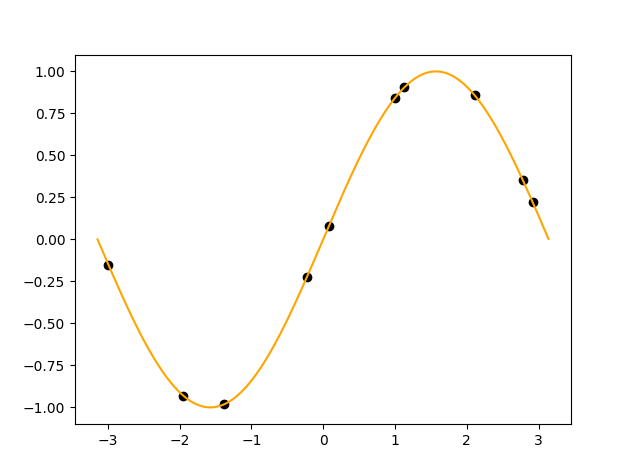
\includegraphics{lagrangepng.png}
	
	\gr Παρακάτω το σφάλμα προσέγγισης για \en 200 \gr σημεία στο [−π, π] καλώντας την \en plotForDiffLagrange. \gr

	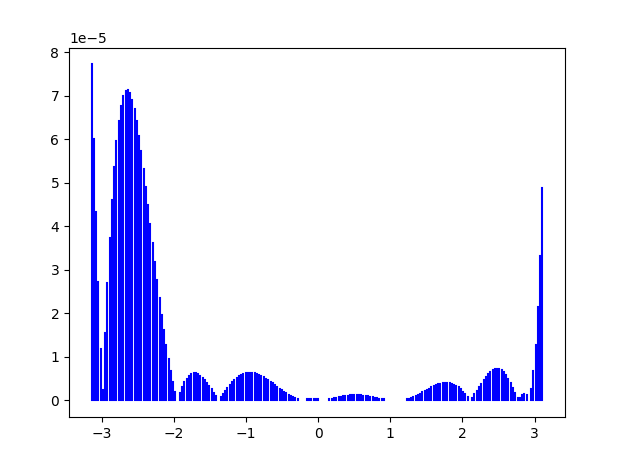
\includegraphics{lagrangeDiff.png}
	
	Η χειρότερη προσέγγιση ήταν ίση με \[ 7.72 * 10^{-5} \] ενώ η καλύτερη
	\[ 1.19 * 10 ^ {-9} \] Επιτεύχθηκαν 4 ψηφία ακρίβειας αν πάρουμε την
	άπειρη νόρμα για αυτά τα 200 σημεία.
	
	\subsubsection{Προσέγγιση ελαχίστων
	τετραγώνων}\label{ux3c0ux3c1ux3bfux3c3ux3adux3b3ux3b3ux3b9ux3c3ux3b7-ux3b5ux3bbux3b1ux3c7ux3afux3c3ux3c4ux3c9ux3bd-ux3c4ux3b5ux3c4ux3c1ux3b1ux3b3ux3ceux3bdux3c9ux3bd}

	\gr Παρακάτω μια γραφική παράσταση της προσέγγισης ελαχίστων τετραγώνων χρησιμοποιόντας την \en plotLeastSquares \gr για πολυώνυμο 3ου βαθμού. Με πορτοκαλί είναι οι τιμές της προσέγγισης σε διάφορα σημεία για να φαίνεται ομαλή και με μπλε είναι οι τιμές του ημίτονου για τα ίδια διάφορα σημεία. Με μάυρο είναι τα σημεία που χρησιμοποιήθηκαν για να φτιαχτεί η προσέγγιση. \gr
	
	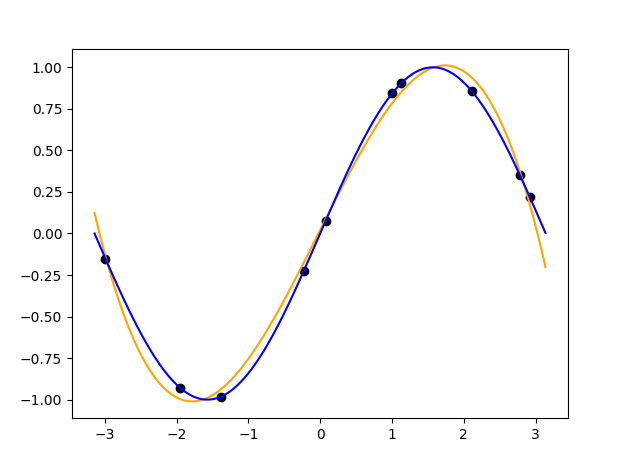
\includegraphics{leastSquares.png}
	
	\gr Παρακάτω το σφάλμα προσέγγισης για \en 200 \gr σημεία στο [−π, π] καλώντας την \en plotForDiffLeastSquares \gr για πολυώνυμο 3ου βαθμού. \gr
	\en
	
	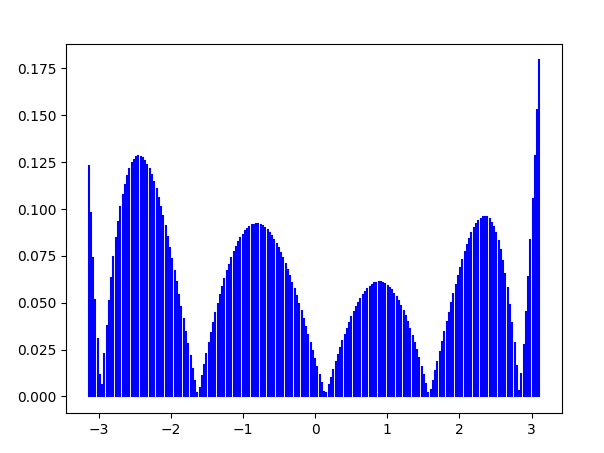
\includegraphics{LeastSqauresDiff.png}
	\gr
	Η χειρότερη προσέγγιση ήταν ίση με \[ 0.179302 \] ενώ η καλύτερη
	\[ 0.001703 \] Επιτεύχθηκε 1 ψηφίο ακρίβειας αν πάρουμε την άπειρη νόρμα
	για αυτά τα 200 σημεία.
	
	\subsection{Άσκηση 7}\label{ux3acux3c3ux3baux3b7ux3c3ux3b7-7}
	
	Οι μετοχές που επέλεξα έχουν τα σύμβολα ΕΥΔΑΠ και ΚΑΡΕΛ. Τα γενέθλια μου
	είναι στις 8/2. Επομένως οι 10 μέρες που επέλεχθηκαν είναι και για τις
	δύο μετοχές οι εξής: (\emph{07/2/2020, 06/2/2020, 05/2/2020, 04/2/2020,
	03/2/2020, 30/1/2020, 29/1/2020, 28/1/2020, 27/1/2020, 24/1/2020}) ενώ
	οι 5 μέρες μετά: (\emph{14/2/2020, 13/2/2020, 12/2/2020, 11/2/2020,
	10/2/2020}). Για κάθε μετοχή και βαθμό προσέγγισης θα δίνεται ένας πίνακας που για κάθε μέρα θα αναφέρει την ημερομηνία, την πραγματική τιμή κλεισίματος, την τιμή προσέγγισης από τον αλγόριθμο και την απόλυτη τιμή της διαφοράς των δύο τελευταίων τιμών. Κάθε πίνακας θα συνοδεύεται με μια βοηθητική γραφική παράστηαση όπου με πορτοκαλί χρώμα θα είναι η προσεγγιστική συνάρτηση ενώ με μαύρο θα είναι τα σημεία που χρησιμοποιήθηκαν από τον αλγόριθμο των ελάχιστων τετραγώνων. Ακόμη με μπλε χρώμα θα είναι οι πραγματικές τιμές των 5 σημείων για τα οποία έγινε η πρόβλεψη. Τέλος θα σχολιάζονται τα αποτελέσματα. (\textbf{Προσοχή:} Μέσα στον κώδικα δεν δίνεται άμεσα η επιλογή να παραχθεί η γραφική παράσταση με ακριβώς αυτό τον τρόπο)
	
	\subsection{Πρώτη μετοχή:
	ΚΑΡΕΛ}\label{ux3c0ux3c1ux3ceux3c4ux3b7-ux3bcux3b5ux3c4ux3bfux3c7ux3ae-ux3baux3b1ux3c1ux3b5ux3bb}
	
	\subsubsection{Προσέγγιση 2ου βαθμού}

	Πίνακα αποτελεσμάτων:

	
	\begin{tabular}{| l | l | l | l |}
	\hline
	Ημερομηνία & Πραγματική τιμή & Τιμή προσέγγισης & Διαφορά
	\\ \hline
	14/2/2020 & 2980000 & 3021575.75758 & 41575.76
	\\ \hline
	13/2/2020 & 2980000 & 3017090.90909 & 37090.91
	\\ \hline
	12/2/2020 & 2980000 & 3012000.0 & 32000.0
	\\ \hline
	11/2/2020 & 2900000 & 3006303.0303 & 106303.03
	\\ \hline
	10/2/2020 & 2920000 & 3000000.0 & 80000.0
	\\ \hline
	07/2/2020 & 2960000 & 2993090.90909 & 33090.91
	\\ \hline
	06/2/2020 & 3000000 & 2985575.75758 & 14424.24
	\\ \hline
	05/2/2020 & 3000000 & 2977454.54545 & 22545.45
	\\ \hline
	04/2/2020 & 3000000 & 2968727.27273 & 31272.73
	\\ \hline
	03/2/2020 & 2980000 & 2959393.93939 & 20606.06
	\\ \hline
	30/1/2020 & 2900000 & 2949454.54545 & 49454.55
	\\ \hline
	29/1/2020 & 2920000 & 2938909.09091 & 18909.09
	\\ \hline
	28/1/2020 & 2920000 & 2927757.57576 & 7757.58
	\\ \hline
	27/1/2020 & 2920000 & 2916000.0 & 4000.0
	\\ \hline
	24/1/2020 & 2920000 & 2903636.36364 & 16363.64
	\\ \hline
	\end{tabular}

	\hfill \break
	
	Γραφική παράσταση:
	
	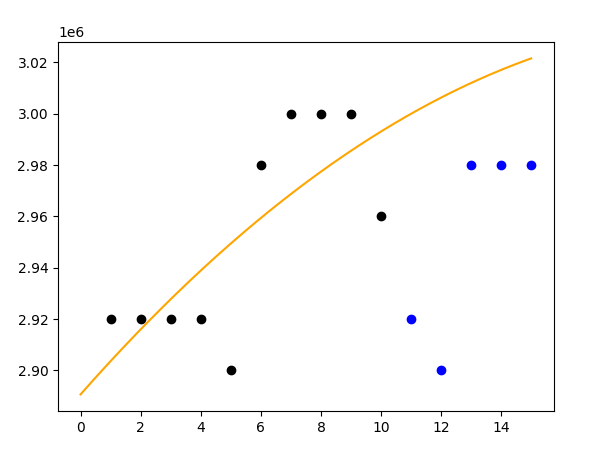
\includegraphics[height=8cm]{karel-2-alt.png}
	
	Σχολιασμός:
	\hfill \break
	
	Στις 10/2 η προσεγγιστική τιμή είναι ίση με 3000000 που έχει απόκλιση 80000 από την πραγματική τιμή εκείνης της ημέρα. Για τις επόμενες προβλέψεις παρατηρούμε πως η ψαλίδα της διαφοράς δεν γίνεται απαγορευτικά μεγάλη με την μεγαλύτερη να είναι αυτή στις 11/2/2020 με τιμή περίπου ίση με 106303. Επίσης παρατηρούμε πως η διαφορά μεταξύ προσέγγισης και πραγματικών τιμών δεν αλλάζει πολύ μεταξύ των γνωστών 10 σημείων και των 5 σημείων για τα οποία έγινε μόνο πρόβλεψη.
	
	


	\subsubsection{Προσέγγιση 3ου βαθμού}
	
	Πίνακα αποτελεσμάτων:

	\begin{tabular}{| l | l | l | l |}
	\hline
	Ημερομηνία & Πραγματική τιμή & Τιμή προσέγγισης & Διαφορά
	\\ \hline
	14/2/2020 & 2980000 & 2229156.17716 & 750843.82
	\\ \hline
	13/2/2020 & 2980000 & 2476895.1049 & 503104.9
	\\ \hline
	12/2/2020 & 2980000 & 2667757.57576 & 312242.42
	\\ \hline
	11/2/2020 & 2900000 & 2808363.63636 & 91636.36
	\\ \hline
	10/2/2020 & 2920000 & 2905333.33333 & 14666.67
	\\ \hline
	07/2/2020 & 2960000 & 2965286.71329 & 5286.71
	\\ \hline
	06/2/2020 & 3000000 & 2994843.82284 & 5156.18
	\\ \hline
	05/2/2020 & 3000000 & 3000624.70862 & 624.71
	\\ \hline
	04/2/2020 & 3000000 & 2989249.41725 & 10750.58
	\\ \hline
	03/2/2020 & 2980000 & 2967337.99534 & 12662.0
	\\ \hline
	30/1/2020 & 2900000 & 2941510.48951 & 41510.49
	\\ \hline
	29/1/2020 & 2920000 & 2918386.94639 & 1613.05
	\\ \hline
	28/1/2020 & 2920000 & 2904587.41259 & 15412.59
	\\ \hline
	27/1/2020 & 2920000 & 2906731.93473 & 13268.07
	\\ \hline
	24/1/2020 & 2920000 & 2931440.55944 & 11440.56
	\\ \hline
	\end{tabular}

	\hfill \break
	
	Γραφική παράσταση:
	
	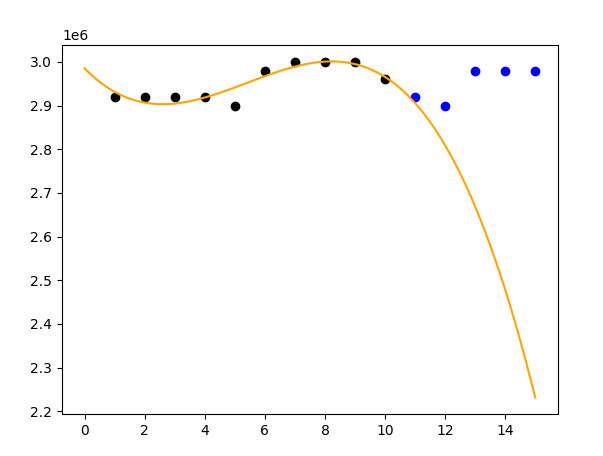
\includegraphics[height=8cm]{karel-3-alt.png}
	
	Σχολιασμός:
	\hfill \break
	
	Στις 10/2 η προσεγγιστική τιμή είναι περίπου ίση με 2905333.3 και έχει απόκλιση περίπου ίση με 14666.67 από την πραγματική τιμή εκείνης της ημέρας. Για τις επόμενες προβλέψεις
	παρατηρούμε πως η ψαλίδα της διαφοράς ανοίγει πολύ για τις 3 τελευταίες προβλέψεις με μεγαλύτερη απόκλιση να έχει η πρόβλεψη για τις 14/2/2020 περίπου ίση με 750843.82. Σε σχέση με την προσέγγιση 2ου βαθμού οι προσέγγισεις για τιμές γνωστές στον αλγόριθμο είναι καλύτερες ενώ για τιμές άγνωστες είναι χειρότερες.
	
	

	\subsubsection{Προσέγγιση 4ου βαθμού}
	
	Πίνακα αποτελεσμάτων:

	\begin{tabular}{| l | l | l | l |}
		\hline
		Ημερομηνία & Πραγματική τιμή & Τιμή προσέγγισης & Διαφορά
		\\ \hline
		14/2/2020 & 2980000 & 898414.91841 & 2081585.08
		\\ \hline
		13/2/2020 & 2980000 & 1682377.62238 & 1297622.38
		\\ \hline
		12/2/2020 & 2980000 & 2235757.57576 & 744242.42
		\\ \hline
		11/2/2020 & 2900000 & 2605454.54545 & 294545.45
		\\ \hline
		10/2/2020 & 2920000 & 2833333.33333 & 86666.67
		\\ \hline
		07/2/2020 & 2960000 & 2956223.77622 & 3776.22
		\\ \hline
		06/2/2020 & 3000000 & 3005920.74592 & 5920.75
		\\ \hline
		05/2/2020 & 3000000 & 3009184.14918 & 9184.15
		\\ \hline
		04/2/2020 & 3000000 & 2987738.92774 & 12261.07
		\\ \hline
		03/2/2020 & 2980000 & 2958275.05828 & 21724.94
		\\ \hline
		30/1/2020 & 2900000 & 2932447.55245 & 32447.55
		\\ \hline
		29/1/2020 & 2920000 & 2916876.45688 & 3123.54
		\\ \hline
		28/1/2020 & 2920000 & 2913146.85315 & 6853.15
		\\ \hline
		27/1/2020 & 2920000 & 2917808.85781 & 2191.14
		\\ \hline
		24/1/2020 & 2920000 & 2922377.62238 & 2377.62
		\\ \hline
		
	\end{tabular}

	\hfill \break
	
	Γραφική παράσταση:
	
	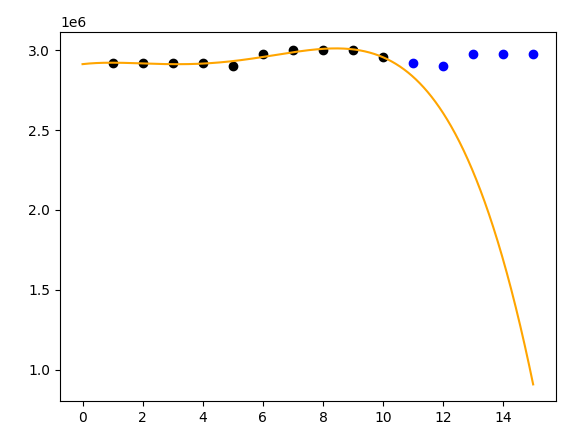
\includegraphics[height=8cm]{karel-4-alt.png}
	
	Σχολιασμός:
	\hfill \break
	
	Στις 10/2 η προσεγγιστική τιμή είναι περίπου ίση με 2833333.3 και έχει απόκλιση περίπου ίση με 86666.67 από την πραγματική τιμή εκείνης της ημέρας. Για τις επόμενες προβλέψεις
	παρατηρούμε πως η ψαλίδα της διαφοράς ανοίγει ακόμη περισσότερο από αυτή της προσέγγισης 3ου βαθμού για τις 3 τελευταίες προβλέψεις με μεγαλύτερη απόκλιση να έχει η πρόβλεψη για τις 14/2/2020 περίπου ίση με 2081585.08. Σε σχέση με την προσέγγιση 3ου βαθμού οι προσέγγισεις για τιμές γνωστές στον αλγόριθμο είναι καλύτερες ενώ για τιμές άγνωστες είναι χειρότερες.
	

	\subsection{Δεύτερη μετοχή:
	ΕΥΔΑΠ}\label{ux3c0ux3c1ux3ceux3c4ux3b7-ux3bcux3b5ux3c4ux3bfux3c7ux3ae-ux3baux3b1ux3c1ux3b5ux3bb}
	
	\subsubsection{Προσέγγιση 2ου βαθμού}
	
	Πίνακα αποτελεσμάτων:
	
	\begin{tabular}{| l | l | l | l |}
		\hline
		Ημερομηνία & Πραγματική τιμή & Τιμή προσέγγισης & Διαφορά
		\\ \hline
		14/2/2020 & 75300 & 74465.60606 & 834.39
		\\ \hline
		13/2/2020 & 74200 & 74452.12121 & 252.12
		\\ \hline
		12/2/2020 & 75200 & 74463.63636 & 736.36
		\\ \hline
		11/2/2020 & 74100 & 74500.15152 & 400.15
		\\ \hline
		10/2/2020 & 73200 & 74561.66667 & 1361.67
		\\ \hline
		07/2/2020 & 74000 & 74648.18182 & 648.18
		\\ \hline
		06/2/2020 & 75300 & 74759.69697 & 540.3
		\\ \hline
		05/2/2020 & 75600 & 74896.21212 & 703.79
		\\ \hline
		04/2/2020 & 75300 & 75057.72727 & 242.27
		\\ \hline
		03/2/2020 & 74400 & 75244.24242 & 844.24
		\\ \hline
		30/1/2020 & 74800 & 75455.75758 & 655.76
		\\ \hline
		29/1/2020 & 76400 & 75692.27273 & 707.73
		\\ \hline
		28/1/2020 & 76000 & 75953.78788 & 46.21
		\\ \hline
		27/1/2020 & 76000 & 76240.30303 & 240.3
		\\ \hline
		24/1/2020 & 76700 & 76551.81818 & 148.18
		\\ \hline
	\end{tabular}

	\hfill \break
	
	Γραφική παράσταση:
	
	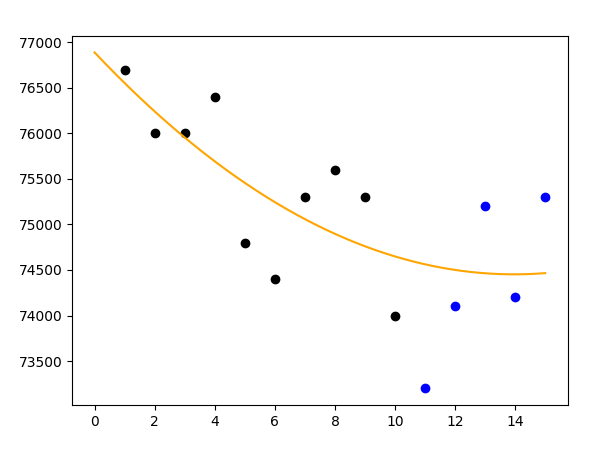
\includegraphics[height=8cm]{eydap-2-alt.png}
	
	Σχολιασμός:
	\hfill \break
	
		
	Στις 10/2 η προσεγγιστική τιμή είναι περίπου ίση με 74561.7 και έχει απόκλιση περίπου ίση με 1361.67 από την πραγματική τιμή εκείνης της ημέρας και είναι η μεγαλύτερη από όλες τις αποκλίσεις. Για τις επόμενες προβλέψεις παρατηρούμε πως η ψαλίδα της διαφοράς παραμένει σταθερή. Επίσης παρατηρούμε πως η διαφορά μεταξύ προσέγγισης και πραγματικών τιμών δεν αλλάζει πολύ μεταξύ των γνωστών 10 σημείων και των 5 σημείων για τα οποία έγινε μόνο πρόβλεψη.
	

	\subsubsection{Προσέγγιση 3ου βαθμού}
	
	Πίνακα αποτελεσμάτων:
	
	\begin{tabular}{| l | l | l | l |}
	\hline
	Ημερομηνία & Πραγματική τιμή & Τιμή προσέγγισης & Διαφορά
	\\ \hline
	14/2/2020 & 75300 & 67392.42424 & 7907.58
	\\ \hline
	13/2/2020 & 74200 & 69630.30303 & 4569.7
	\\ \hline
	12/2/2020 & 75200 & 71390.90909 & 3809.09
	\\ \hline
	11/2/2020 & 74100 & 72733.33333 & 1366.67
	\\ \hline
	10/2/2020 & 73200 & 73716.66667 & 516.67
	\\ \hline
	07/2/2020 & 74000 & 74400.0 & 400.0
	\\ \hline
	06/2/2020 & 75300 & 74842.42424 & 457.58
	\\ \hline
	05/2/2020 & 75600 & 75103.0303 & 496.97
	\\ \hline
	04/2/2020 & 75300 & 75240.90909 & 59.09
	\\ \hline
	03/2/2020 & 74400 & 75315.15152 & 915.15
	\\ \hline
	30/1/2020 & 74800 & 75384.84848 & 584.85
	\\ \hline
	29/1/2020 & 76400 & 75509.09091 & 890.91
	\\ \hline
	28/1/2020 & 76000 & 75746.9697 & 253.03
	\\ \hline
	27/1/2020 & 76000 & 76157.57576 & 157.58
	\\ \hline
	24/1/2020 & 76700 & 76800.0 & 100.0
	\\ \hline
	\end{tabular}

	\hfill \break
	
	Γραφική παράσταση:
	
	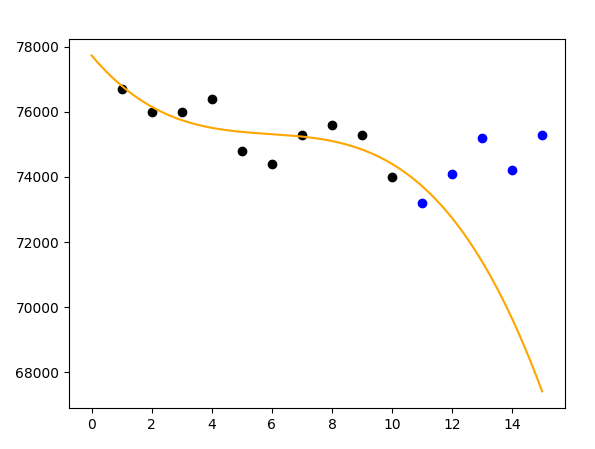
\includegraphics[height=8cm]{eydap-3-alt.png}
	
	Σχολιασμός:
	\hfill \break
	
	Στις 10/2 η προσεγγιστική τιμή είναι περίπου ίση με 73716.7 και έχει απόκλιση περίπου ίση με 516.67 από την πραγματική τιμή εκείνης της ημέρας. Για τις επόμενες προβλέψεις
	παρατηρούμε πως η ψαλίδα της διαφοράς ανοίγει πολύ για τις 3 τελευταίες προβλέψεις με μεγαλύτερη απόκλιση να έχει η πρόβλεψη για τις 14/2/2020 περίπου ίση με 7907.58. Σε σχέση με την προσέγγιση 2ου βαθμού οι προσέγγισεις για τιμές γνωστές στον αλγόριθμο είναι καλύτερες ενώ για τιμές άγνωστες είναι χειρότερες.

	\subsubsection{Προσέγγιση 4ου βαθμού}
	
	Πίνακα αποτελεσμάτων:
	
	\begin{tabular}{| l | l | l | l |}
		\hline
	Ημερομηνία & Πραγματική τιμή & Τιμή προσέγγισης & Διαφορά
	\\ \hline
	14/2/2020 & 75300 & 18875.81585 & 56424.18
	\\ \hline
	13/2/2020 & 74200 & 40663.51981 & 33536.48
	\\ \hline
	12/2/2020 & 75200 & 55640.90909 & 19559.09
	\\ \hline
	11/2/2020 & 74100 & 65335.60606 & 8764.39
	\\ \hline
	10/2/2020 & 73200 & 71091.66667 & 2108.33
	\\ \hline
	07/2/2020 & 74000 & 74069.58042 & 69.58
	\\ \hline
	06/2/2020 & 75300 & 75246.2704 & 53.73
	\\ \hline
	05/2/2020 & 75600 & 75415.09324 & 184.91
	\\ \hline
	04/2/2020 & 75300 & 75185.83916 & 114.16
	\\ \hline
	03/2/2020 & 74400 & 74984.73193 & 584.73
	\\ \hline
	30/1/2020 & 74800 & 75054.4289 & 254.43
	\\ \hline
	29/1/2020 & 76400 & 75454.02098 & 945.98
	\\ \hline
	28/1/2020 & 76000 & 76059.03263 & 59.03
	\\ \hline
	27/1/2020 & 76000 & 76561.42191 & 561.42
	\\ \hline
	24/1/2020 & 76700 & 76469.58042 & 230.42
	\\ \hline
	\end{tabular}

	\hfill \break
	
	Γραφική παράσταση:
	
	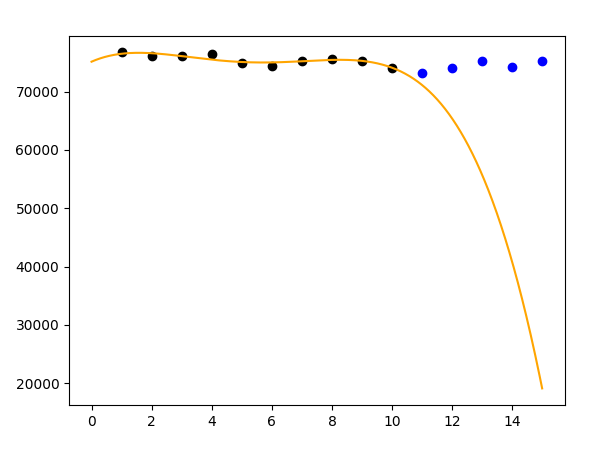
\includegraphics[height=8cm]{eydap-4-alt.png}
	
	Σχολιασμός:
	\hfill \break
	
	Στις 10/2 η προσεγγιστική τιμή είναι περίπου ίση με 71091.7 και έχει απόκλιση περίπου ίση με 2108.33 από την πραγματική τιμή εκείνης της ημέρας. Για τις επόμενες προβλέψεις
	παρατηρούμε πως η ψαλίδα της διαφοράς ανοίγει ακόμη περισσότερο από αυτή της προσέγγισης 3ου βαθμού για τις 4 τελευταίες προβλέψεις με μεγαλύτερη απόκλιση να έχει η πρόβλεψη για τις 14/2/2020 περίπου ίση με 56424.18. Σε σχέση με την προσέγγιση 3ου βαθμού οι προσέγγισεις για τιμές γνωστές στον αλγόριθμο είναι καλύτερες ενώ για τιμές άγνωστες είναι χειρότερες.
	
	\subsection{Σχολιασμός}
	
	Παρατηρώντας τις προσεγγίσεις και για τις δύο μετοχές καταλήγουμε στο συμπέρασμα πως (για τουλάχιστον τα συγκεκριμένα παραδείγματα) όσο μεγαλύτερος είναι ο βαθμός του πολυωνύμου προσέγγισης τόσο μεγαλύτερη ακρίβεια υπάρχει για τις τιμές γνωστές στον αλγόριθμο ελαχίστων τετραγώνων και τόσο μικρότερη ακρίβεια για άγνωστες τιμές. Ίσως αυτό να είναι ένα φαινόμενο υπερεκπαίδευσης.
	
\end{document}
